% -*- Mode:TeX -*-

%% IMPORTANT: The official thesis specifications are available at:
%%            http://libraries.mit.edu/archives/thesis-specs/
%%
%%            Please verify your thesis' formatting and copyright
%%            assignment before submission.  If you notice any
%%            discrepancies between these templates and the 
%%            MIT Libraries' specs, please let us know
%%            by e-mailing thesis@mit.edu

%% The documentclass options along with the pagestyle can be used to generate
%% a technical report, a draft copy, or a regular thesis.  You may need to
%% re-specify the pagestyle after you \include  cover.tex.  For more
%% information, see the first few lines of mitthesis.cls. 

%\documentclass[12pt,vi,twoside]{mitthesis}
%%
%%  If you want your thesis copyright to you instead of MIT, use the
%%  ``vi'' option, as above.
%%
%\documentclass[12pt,twoside,leftblank]{mitthesis}
%%
%% If you want blank pages before new chapters to be labelled ``This
%% Page Intentionally Left Blank'', use the ``leftblank'' option, as
%% above. 

\documentclass[oneside,letterpaper,12pt,spanish]{report}
\usepackage{lgrind}
%% These have been added at the request of the MIT Libraries, because
%% some PDF conversions mess up the ligatures.  -LB, 1/22/2014
\usepackage{cmap}
\usepackage[T1]{fontenc}
\usepackage[utf8]{inputenc} %%%Para poner acentos directamente
\usepackage{latexsym}
\usepackage{lmodern}
\usepackage{amsmath}
\usepackage{setspace}
%\usepackage[spanish]{babel} % division de silabas en español.
%\usepackage{ucs}
%\usepackage[utf8]{inputenc} %%%Para poner acentos directamente

%\usepackage[T1]{fontenc}
\usepackage{fancyhdr}
%\usepackage{babel}
\usepackage{makeidx}
\usepackage{graphics}  
\usepackage{algorithm}
%\usepackage{algorithmic}
\usepackage[dvips]{graphicx}
\usepackage{latexsym}
\usepackage{amssymb} 
\usepackage{amsthm}
\usepackage{url}
\usepackage{color}
\usepackage{float}

\renewcommand{\chaptername}{Capítulo}
\renewcommand{\contentsname}{Contenidos}
\renewcommand{\listfigurename}{Lista de figuras}
\renewcommand{\bibname}{Bibliografia}
\addtolength{\textwidth}{1cm} % Ancho del texto

% traducción de algunos nombres del paquete algorithm
%\floatname{algorithm}{Algoritmo}
%\renewcommand{\listalgorithmname}{Indice de algoritmos}
\newcommand{\mucalculo}{$\mu$-Cálculo}
% Definiciones
\newtheorem{definition}{Definición}[section]

%Ejemplos
\newtheorem{ejemplo}{\normalfont \rule{0.2in}{0.11in}  {\rm Ejemplo }} [section]

%Casos de las reglas de reconstraccion
\newtheorem{caso}{\large {\rm Caso}}
 

%SUBCasos de las reglas de reconstraccion
\newtheorem{subcaso}{\large {\rm Caso}} [caso]

     
% Teoremas
\newtheorem{theorem}{Teorema}[section]

% Lemmas
\newtheorem{lema}{Lema}[section]

%%%%%%%%%%%%%%%% DEFINICIONES DE ALGUNOS COMANDOS Y AMBIENTES %%%%%%%%%%%%%%%

\newcounter{ruleAGcounter}
\newenvironment{AG}
{
 \setcounter{ruleAGcounter}{0} \begin{center} \begin{figure}[!hb]
 \rule{\textwidth}{.5pt} \footnotesize
}
{\normalsize \rule{\textwidth}{.5pt} \end{figure} \end{center}}
 
\newcommand{\newproduction}[2]{$p_\arabic{ruleAGcounter}$:
            \emph{#1} $\rightarrow$ \emph{#2}
            \addtocounter{ruleAGcounter}{1}\\}

%Por ahora al pedo esta lo que sigue
\newenvironment{micaso}[1][2] {\begin{caso} \textnormal{#1}} {\end{caso}}

%\newenvironment{proof}[1][Prueba]{}
 
\newcommand{\attribution}[1]{\hspace*{2cm}\emph{#1} \\} 

%Letra de los Estados
\newcommand{\letraEstado} [1] {\texttt{#1}}
%Letra de lso Diagramas de Clases
\newcommand{\letraDC} [1] {\texttt{#1}}
%Letra de las Funcionalidades
\newcommand{\letraFunc} [1] {\normalsize{#1}}
%Letra  del texto OR y AND
\newcommand{\letraORAND} [1] {\texttt{#1}}
%Color del texto
\newcommand{\textocolor} [1] {\textcolor{black}{#1}}
%Color del texto 2
\newcommand{\textocolorDos} [1] {\textcolor{black}{#1}}
%Color del texto 3
\newcommand{\textocolorTres} [1] {\textcolor{black}{#1}}


%letras de los elementos Ecore
\newcommand{\letraEcore} [1] {\texttt{#1}}
\newcommand{\letraRelaciones} [1] {\textbf{#1}}

\makeatother
\makeindex
 
%============================================================================

\pagestyle{plain}

%% This bit allows you to either specify only the files which you wish to
%% process, or `all' to process all files which you \include.
%% Krishna Sethuraman (1990).

\typein [\files]{Enter file names to process, (chap1,chap2 ...), or `all' to
process all files:}
\def\all{all}
\ifx\files\all \typeout{Including all files.} \else \typeout{Including only \files.} \includeonly{\files} \fi

\begin{document}
\raggedbottom

\title{
UNIVERSIDAD NACIONAL DE RIO CUARTO\\
$\;$\\
$\;$\\
\small{Trabajo de tesis para la obtenci\'on del grado de Licenciatura en Ciencias de la Computaci\'on}
$\;$\\$\;$\\
\Large{\textbf{ T\'itulo : Un Verificador de Modelos Funcional para \mucalculo}}
} 

\author{
                        Autor\\
                        Luciano Putruele\\
                        \\
                 Director de Tesis: \emph{Dr. Pablo F. Castro}\\ 
                 Co-Director de Tesis: \emph{Dr. Germán Regis}\\ 
}

\date{Rio Cuarto, Argentina\\ Abril 2016}

 
\maketitle
 

%Para dejar una página en blanco
\newpage
\mbox{}
\thispagestyle{empty} % para que no se numere esta página

%Incluye el abstact y los Agradecimientos.

% $Log: abstract.tex,v $
% Revision 1.1  93/05/14  14:56:25  starflt
% Initial revision
% 
% Revision 1.1  90/05/04  10:41:01  lwvanels
% Initial revision
% 
%
%% The text of your abstract and nothing else (other than comments) goes here.
%% It will be single-spaced and the rest of the text that is supposed to go on
%% the abstract page will be generated by the abstractpage environment.  This
%% file should be \input (not \include 'd) from cover.tex.
\chapter*{Resumen}
\pagenumbering{roman}
\addcontentsline{toc}{chapter}{Resumen} % si queremos que aparezca en el índice

En esta tesis desarrollaremos una herramienta de verificación de modelos (\emph Model \emph Checking), llamada MC2 (Mu Cálculus Model Checker, o MCMC, de ahi MC2), sobre modelos de sistemas formalizados en un lenguaje de descripción simple que también será desarrollado en este trabajo. La herramienta de verificación se encargará de, valga la redundancia, verificar propiedades, caracterizadas en la forma de la lógica temporal Cálculo-$\mu$ (o cálculo-Mu), sobre algún modelo descripto. Cabe destacar que tanto el lenguaje de descripción de modelos como el verificador forman parte de la misma herramienta, incluso las propiedades a verificar se deben especificar en la descripción.

Adicionalmente, los descripciones MC2 se basan en la definición de reglas de transición usando proposiciones lógicas atómicas con lo cual es transparente ver la estructura del modelo como una máquina de transición de estados más allá de que internamente se los trata simbólicamente como fórmulas para mejorar el rendimiento.

A todo esto, el metalenguaje utilizado para el desarrollo de estas herramientas es Haskell. Esto también significó una motivación para el desarrollo de esta tesis ya que la utilización de un lenguaje funcional como Haskell para el desarrollo de la herramienta en su totalidad, en lugar de la utilización lenguajes imperativos u orientados a objetos, da un enfoque distinto al comportamiento de la herramienta.

Lo que se propone con este proyecto es explorar otras alternativas para especificar propiedades que un modelo deba satisfacer, siendo la alternativa en este trabajo el Cálculo Mu, en vez de las lógicas temporales más utilizadas en este tipo de herramientas, como ser LTL, CTL y CTL*, ya que esto trae la ventaja de que el Cálculo-Mu es más expresivo que los anteriormente nombrados. MC2 puede servir como herramienta de bajo nivel, en el sentido de que se puede extraer una descripción MC2 a partir de modelos de mas alto nivel, y asi mismo, propiedades en lógicas temporales de más alto nivel, para asi despues usar el verificador MC2 sobre la descripción extraida.


%\emph{Palabras clave}: .

%\thispagestyle{empty} % para que no se numere esta página
%\end{abstract}

\chapter*{Agradecimientos}
\addcontentsline{toc}{chapter}{Agradecimientos} % si queremos que aparezca en el índice
%\thispagestyle{empty} 
{\sl Agradezco a la universidad, el departamento de computación, y en especial a mi familia y mis amigos, esto no seria posible sin ellos.}


%\thispagestyle{empty} 
\listoffigures
%\thispagestyle{empty} 
\addcontentsline{toc}{chapter}{Lista de figuras} % para que aparezca en el indice de contenidos
%\thispagestyle{empty} 
%Las siguintes 3 lineas es para sacarle la numeracion de paginas al Indice
%\addtocontents{toc}{\protect\thispagestyle{empty}}
\tableofcontents %put toc in
%\thispagestyle{empty} 
%\cleardoublepage %start new page


%\addtolength{\headwidth}{1cm} % Ancho del encabezado (fancy headers)
\renewcommand{\sectionmark}[1]{}
\renewcommand{\chaptermark}[1]{\markboth{#1}{}} % capíitulo en minísculas

%En la Introduccion se resetea el contador de paginas y el estilo de fuente de los numeros.

%% This is an example first chapter.  You should put chapter/appendix that you
%% write into a separate file, and add a line \include{yourfilename} to
%% main.tex, where `yourfilename.tex' is the name of the chapter/appendix file.
%% You can process specific files by typing their names in at the 
%% \files=
%% prompt when you run the file main.tex through LaTeX.
\chapter{Introducción}
\pagenumbering{arabic}
\noindent La verificación de modelos (\emph{model checking}) es una técnica automática para verificar modelos de sistemas con una cantidad finita de estados, por ejemplo protocolos de comunicación y diseños de circuitos, entre otros. En general, la aplicación de esta técnica consta de una caracterización del modelo en términos de algún tipo de sistema de transición de estados y la especificación de la propiedad a analizar en algún tipo de lenguaje formal, comúnmente algún tipo de lógica temporal.\\
\\
\noindent Se utiliza una búsqueda eficiente para determinar automáticamente si las especificaciones son satisfechas por el grafo \cite{Clarke:5}. Esta técnica fue desarrollada originalmente en 1981 por Clarke y Emerson. Esta técnica tiene varias ventajas importantes sobre probadores de teoremas para verificación de circuitos y protocolos. La más importante es que es automática. Normalmente, el usuario provee una representación de alto nivel del modelo y una especificación de la propiedad que se desea verificar. El model checker terminará devolviendo la respuesta True indicando que el modelo satisface la especificación o dará una traza de ejecución a modo de contra-ejemplo si el modelo no satisface la propiedad. Esta es una propiedad muy importante a la hora de encontrar bugs sutiles.

\section{Objetivos}
El objetivo principal de este proyecto es proveer una herramienta de verificación de modelos puramente funcional además de explorar otras alternativas para especificar propiedades que un modelo deba satisfacer, siendo la alternativa en este trabajo el {\mucalculo}, un lenguaje altamente expresivo, lo cuál trae la ventaja de que propiedades descritas en muchos otros tipos de lógicas temporales pueden ser descritos también por el {\mucalculo}. En cuanto a la aplicación práctica de la herramienta, la misma esta planeada para verificar propiedades en lógicas donde el problema de la verificación de modelos pueda ser reducida a {\mucalculo}, por ejemplo dCTL \cite{Castro:9}, una lógica temporal deóntica usada para especificar propiedades sobre sistemas tolerantes a fallos.

\section{Estructura}
En el capítulo 2 analizaremos conceptos básicos para la comprensión de esta tesis, conceptos como la verificación de modelos, representación de estos modelos, el concepto de lógicas temporales, y en particular, el {\mucalculo}.
En el capítulo 3 veremos formas de representar los datos de una manera más concisa e introduciremos la noción de verificación simbólica de modelos.
En el capítulo 4 nos adentramos en la herramienta MC2, su lenguaje de descripción de modelos y su verificador de modelos. Se entra en detalle con la sintaxis y la semántica del lenguaje. Para terminar, se analizarán cuestiones de diseño e implementación de la herramienta. 
En el capítulo 5 aplicaremos la herramienta a algunos casos de estudio concretos a modo de ejemplificación del uso práctico de esta herramienta.

\section{Disposición de la herramienta}

La herramienta MC2 se puede encontrar en el siguiente repositorio:\\
\\
https://github.com/lputruele/MC2-Mu-Calculus-Model-Checker




%% This is an example first chapter.  You should put chapter/appendix that you
%% write into a separate file, and add a line \include{yourfilename} to
%% main.tex, where `yourfilename.tex' is the name of the chapter/appendix file.
%% You can process specific files by typing their names in at the 
%% \files=
%% prompt when you run the file main.tex through LaTeX.
\chapter{Conceptos preliminares}

La verificación de modelos o model checking es una técnica automática de verificación de propiedades sobre sistemas con una cantidad finita de estados. Es una alternativa interesante con respecto al testing o las simulaciones ya que a diferencia de estas técnicas, el model checking hace una prueba exhaustiva del sistema, es decir, analiza todas las trazas posibles de la ejecución del sistema en cuestión. Sin embargo, esto trae un problema, esto es el problema de la explosión de estados. Esto ocurre en sistemas con muchas interacciones internas, y que pueden hacer crecer exponencialmente el espacio de estados posibles del sistema, ya que la prueba es exhaustiva no se puede ignorar ningún estado posible.
En los últimos años se ha logrado un gran progreso en cómo lidiar con este problema mediante formas más compactas de representar al sistema, como por ejemplo, una representación simbólica.

El proceso del model checking consta de varias tareas:

Modelado: Lo primero es convertir el modelo de un sistema en un formalismo aceptado por la herramienta de verificación de modelos.

Especificación: Es necesario expresar de alguna forma las propiedades que necesitan ser verificadas en el modelo. En general estas propiedades se dan en alguna lógica formal, particularmente lógicas temporales ya que estas pueden expresar comportamientos futuros del sistema.

Verificación: Dado el modelo y la especificación, la tarea de verificar significa explorar exhaustivamente todos los estados posibles del sistema para llegar a la conclusión de que el mismo satisface la especificación o no, en este último caso se suele dar también una traza de error, lo cual ayuda al programador para encontrar fallas en el sistema. Sin embargo, la causa de que el modelo no haya pasado la verificación puede deberse a una especificación incorrecta.


\section{Modelado de sistemas}
En esta sección veremos cómo representar un modelo explícitamente mediante una estructura de Kripke, más tarde veremos otra forma de representación llamada simbólica que representa el modelo mediante una fórmula lógica de primer orden.

Sea $AP$ un conjunto de proposiciones atómicas, una estructura de Kripke $M$ sobre $AP$ es una cuatro-upla $M = (S, S_{0}, R, L)$ donde
\newline1. $S$ es un conjunto finito de estados.
\newline2. $S_{0} \in S$ es el conjunto de estados iniciales.
\newline3. $R \in S \times S$ es una relación de transición total, es decir para cada estado $s \in S$ existe un estado $s' \in S$ tal que $R(s,s')$ vale.
\newline4. $L \colon S \to 2^{AP}$ es una función que etiqueta a cada estado con el conjunto de proposiciones atómicas que son verdaderas en ese estado.
Un camino en la estructura $M$ desde un estado $s$ es una secuencia infinita de estados $p = s_{0}, s_{1}, s_{2}, s_{3}, ...$, tal que $s = s_{0}$ y $R(s_{i},s_{i+1})$ vale para todo $i>0$.

Sea $V = {v_{1}, v_{2}, ..., v_{n}}$ el conjunto de variables del sistema y sea $D$ el dominio, llamaremos una valuación de $V$ a una función que asocia a cada variable de $V$ un valor de $D$.

Un estado del sistema se puede representar como una valuación de las variables del sistema. Una proposición atómica de la forma $v = d$ donde $v \in V$ y $d \in D$ será verdadera en un estado $s$ si y solo si $s(v) = d$.
Dada una valuación, podemos escribir una fórmula que sea verdadera precisamente para esa valuación, por ejemplo si tenemos $V = \{x,y,z\}$ y la valuación $(x \gets True, y \gets True, z \gets False)$ entonces derivamos la fórmula $(x \land y \land !z)$. En general, una fórmula puede ser verdadera para varias valuaciones. Si adoptamos la convención de que una fórmula representa el conjunto de todas las valuaciones que la hacen verdadera, entonces podremos describir ciertos conjuntos de estados como fórmulas de primer orden.
En particular, el conjunto de los estados iniciales del sistema puede describirse como una fórmula de primer orden $S_{0}$ sobre las variables en $V$.
Una transición del sistema se puede representar como un par ordenado de valuaciones, de forma similar podemos describir conjuntos de transiciones mediante una formula para ese par, pero para poder expresar la fórmula se necesita una copia $V'$ de $V$ para hablar del \emph siguiente estado, en V' todas las variables estan primadas. Por ejemplo si tenemos una transición $(x \gets True, y \gets True, z \gets False,(x \gets True, y \gets True, z \gets True))$, podemos derivar la fórmula $(x \land y \land !z \land x' \land y' \land z')$.

Consideremos el siguiente ejemplo, tenemos $V = \{x,y,z\}$ y $D = \{True, False\}$, $S_{0} (x,y,z) = (x= True \land y = True \land z = False)$, y tenemos solo una transición: $z := x \land y$, definimos la estructura de kripke de la siguiente manera:

\[S = D \times D \times D\]
\[S_{0} = \{(1, 1, 0)\}\]
\[R = \{((1, 1, 0), (1, 1, 1)), ((1, 1, 1), (1, 1, 1))\}\]
\[L (1, 1, 0) = \{x = 1, y = 1, z = 0\},\]
\[L (1, 1, 1) = \{x = 1, y = 1, z = 1\}\]

El único camino posible en esta estructura partiendo del estado inicial es: (1, 1, 0), (1, 1, 1), (1, 1, 1), (1, 1, 1) …

\section{Especificación de propiedades}

Ahora describiremos una lógica para especificar propiedades deseadas en una estructura de Kripke u otra máquina de transición de estados. La lógica utiliza proposiciones atómicas y operadores como la disyunción y la negación para construir expresiones más complicadas que describan propiedades sobre estados.
La lógica temporal es un formalismo que permite describir secuencias de transiciones entre estados en un sistema reactivo, nos interesa saber si en algún momento se llega a un estado determinado o que nunca se llegue a un deadlock. Para esto introduce nuevos operadores especiales que permiten hablar sobre tiempo. Estos operadores pueden combinarse con los operadores lógicos conocidos.
Analizaremos a continuación una lógica temporal muy potente llamada Cálculo-$\mu$.


\section{Cálculo-$\mu$}

Sea $M = (S, T, L)$ una estructura de Kripke y sea $VAR = {Q, Q1, Q2, …}$ un conjunto de variables relacionales, donde a cada variable relacional se le puede asignar un subconjunto de S, construimos una $\mu$-fórmula como sigue:

-Si $p$ pertenece a $AP$ entonces $p$ es una fórmula.
-Si $Q$ pertenece a $VAR$, $Q$ es una fórmula.
-Si $f$ y $g$ son fórmulas, entonces $\neg f$, $f \lor g$, y $f \land g$ son fórmulas.
-Si $f$ es una fórmula, entonces $\Box f$ y $\Diamond f$ son fórmulas.
-Si $Q \in VAR$ y $f$ es una fórmula entonces $\mu Q.f$ y $\nu Q.f$ son fórmulas

Las variables pueden estar libres o ligadas en una fórmula a través de un operador de punto fijo. Una fórmula cerrada es una fórmula sin variables libres.

El significado intuitivo de $\Diamond f$ es “Es posible realizar una transición a un estado donde f vale“, similarmente $\Box f$ significa “f vale en todos los estados alcanzables por medio de una transición“
Los operadores $\mu$ y $\nu$ expresan puntos fijos menores y mayores respectivamente. El conjunto vacío de estados se denota con $False$ y el conjunto de todos los estados $S$ se denota con $True$.

Ejemplos

-$\nu Z \cdot f \land \Box Z$ se interpreta como “f es verdadera siempre en todo camino”
-$\mu Z \cdot f \lor \Diamond Z$ se interpreta como “existe un camino hacia un estado donde f vale”
-$\nu Z \cdot \Diamond T \land \Box Z$ se interpreta como “no hay estados que no tengan transiciones hacia otros estados”

Formalmente, una fórmula $f$ se interpreta como un conjunto de estados donde $f$ es verdadera, escribimos este conjunto como $[[f]]$ sobre un sistema de transición de estados $M$ y un ambiente $e: VAR \to 2^{S}$, denotaremos $e[Q \gets W]$ como un ambiente que es igual a $e$ solo que $Q$ ahora tiene el valor $W$. el conjunto $[[f]]$ sobre $M$ y $e$ se define recursivamente de la siguiente manera:

\[ [[p]] M e = \{s \mid p \in a L(s)\} \] 
\[ [[Q]] M e = e(Q) \]
\[ [[\neg f]] M e = S \setminus [[f]] M e \]
\[ [[f \land g]] M e = [[f]] M e \cap [[g]] M e \]
\[ [[f \lor g]] M e = [[f]] M e \cup [[g]] M e \]
\[ [[\Diamond f]] M e = \{s \mid \exists t : s \to t \land t \in [[f]] M e\} \]
\[ [[\Box f]] M e = \{s \mid \forall t : s \to t  \rightarrow t \in [[f]] M e\} \]
$[[[\mu Q f]] M e$ es el menor punto fijo del predicado transformador $t:2^{S} \to 2^{S}$ definido como $t(W) = [[f]] M e[Q \gets W] $
$ [[\nu Q f]] M e$ es el mayor punto fijo del predicado transformador $t:2^{S} \to 2^{S}$ definido como $t(W) = [[f]] M e[Q \gets W] $

\chapter{Verificación simbólica de modelos}

El algoritmo de verificación de modelos con estados explícitos para Cálculo-$\mu$ presentado anteriormente tiene un problema, es muy susceptible a que ocurra una explosión en el tamaño del modelo, especialmente si el grafo de transición de estados se extrae de un sistema concurrente con muchos componentes. En esta sección se describe un algoritmo de verificación de modelos simbólicos para Cálculo-$\mu$ que opera sobre estructuras de Kripke, esta vez representadas no de manera explícita, sino de manera simbólica a través de fórmulas lógicas.

\section{Representación de fórmulas lógicas}

Los árboles binarios de decisión ordenados (OBDDs) son formas canónicas de representación de fórmulas lógicas. Son considerablemente mas compactos que las formas normales tradicionales como la forma normal conjuntiva y la forma normal disyuntiva, y pueden ser manipulados eficientemente. Por esto, los OBDDs han sido utilizados ampliamente para una variedad de aplicaciones en el diseño asistido por computadoras, incluyendo simulacion simbólica, verificación de lógica combinatoria y, mas recientemente, verificación de sistemas concurrentes con estados finitos.

Para entender la necesidad de usar OBDDs, consideremos primero los árboles binarios de decisión. Un arbol binario de decisión es un árbol dirigido con raiz que consiste en vertices terminales y no terminales. Cada vertice no terminal v esta etiquetado por una variable $var(v)$ y tiene dos hijos: $izq(v)$ corresponde al caso en que v tenga el valor 0 y $der(v)$ en caso contrario. Cada vértice terminal esta etiquetado por una constante $valor(v)$ la cual es 0 o 1. Un árbol binario de decisión para la fórmula $f(a,b,c) = (a \land b) \lor (a \land c)$ es mostrado en la figura {fig:kripke1}. Uno puede decidir si una asignación particular a las variables hace verdadera la fórmula o no al atravesar el árbol desde la raíz hasta un vertice terminal. Por ejemplo, la asignación ${ a = 1, b = 0, c = 0}$ lleva al vértice terminal 0, por lo tanto la fórmula es falsa para esta asignación.

\begin{figure}[h]
  \centering
  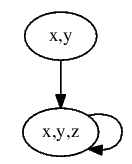
\includegraphics{Figures/kripke.png}
  \caption{Estructura de Kripke para este ejemplo.}
  \label{fig:kripke1}
\end{figure}

\section{Diagramas binarios de decisión}




\chapter{Lenguaje MC2}

MC2 es el verificador de modelos desarrollado en esta tesis, el mismo toma modelos escritos en un lenguaje que tambien llamaremos MC2, el modelo incluye la descripción del sistema y las propiedades que debe satisfacer en Cálculo-$\mu$. El diseño del lenguaje de modelado se centra en la noción de estructuras de Kripke, es decir que con este lenguaje se puede describir el comportamiento del sistema en términos de transiciones de entre estados, y además especificar las propiedades que se desean verificar sobre el modelo. Primero analizaremos la sintaxis y semántica de la parte del lenguaje que se encarga de la descripción del sistema, y luego veremos la sintaxis y semántica de la parte de especificación de propiedades.

\section{Sintaxis}
Sean $p \in AP$,$X \in VName$, entonces la sintaxis de MC2 se define con la siguiente gramática:

\begin{align*}
D &:=\ p \\
   &|\ D;D \\
\\
C &:=\ E->E \\
   &|\ C;C \\
\\
E &:=\ p \\
   &|\ !p \\
   &|\ E,E \\
\\
P &:= F \\
   &|\ P,P \\
\\
F &:=\ p \\
   &|\ :X \\
   &|\ !F \\
   &|\ (F \& F) \\
   &|\ (F | F) \\
   &|\ <>F \\
   &|\ []F \\
   &|\ \%X.F \\
   &|\ \$X.F \\ 
\\
M &:=\ vars\ D\ rules\ C\ init\ E\ check\ P \\
\end{align*}

Usamos la coma $','$ para separar elementos de una lista de expresiones, y , punto y coma $';'$ para separar elementos de una lista de comandos o de declaraciones. La diferencia es sutil pero es importante destacarla para evitar confusión.
Un detalle de implementación muy importante que hace falta destacar es que el parsing de $E$ retorna un ambiente, el cual es una lista de pares $(p,v)$, donde $p \in AP$ y $v \in Bool$. Se puede decir que hay una semántica intermedia para E:

\begin{align*}
[[p]]\ &=\ (p,True)\\
[[!p]]\ &=\ (p,False) \\
[[E0,E1]]\ &=\ [[E0]]\ ++\ [[E1]] \\
\end{align*}

De ahora en mas cuando hablemos de E, hacemos referencia a la lista generada anteriormente.

\section{Semántica} 

\subsection{Semántica informal}

La figura \ref{fig:MC2-1} muestra un ejemplo de una descripción MC2. Aqui representamos una estructura de Kripke con dos estados $s_{0}$,$s_{1}$ donde $L(s_{0}) = \{a,b\}$, $L(s_{1}) = \{a\}$, y $T = \{(s_{0},s_{1}),(s_{1},s_{0}),(s_{1},s_{1})\}$ como el de la figura \ref{fig:kripke4}. En la sección $vars$ se declara el conjunto de proposiciones atómicas del modelo. La sección $rules$ describe las transiciones del sistema. La sección $init$ es donde se señala el valor inicial de las proposiciones atómicas. En la sección $check$ se especifican las propiedades que se desean verificar sobre el modelo en el estado $init$.

\begin{figure}[H]
  \centering
  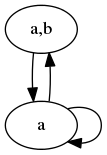
\includegraphics[width=0.2\textwidth]{Figures/kripke4.png}
  \caption{Estructura de Kripke del modelo.}
  \label{fig:kripke4}
\end{figure}

\begin{figure}[H]
  \centering
  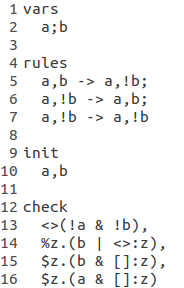
\includegraphics[width=0.35\textwidth]{Figures/modeloMC2-1.png}
  \caption{Ejemplo de descripción MC2.}
  \label{fig:MC2-1}
\end{figure}

Se puede ver que las reglas describen precisamente las tres transiciones del sistema. Aquellas proposiciones que no varian su valor de un estado al siguiente, se las puede obviar en la parte derecha de la regla como se ve en la figura \ref{fig:MC2-2}. Esta descripción es equivalente a la anterior. Intuitivamente podemos pensar la parte izquierda de la regla como el estado corriente y la parte derecha como el siguiente estado, pero en realidad podemos representar mas de una transición con una sola regla. Por ejemplo, la descripción de la figura \ref{fig:MC2-3} modela el sistema de la figura \ref{fig:kripke5}. Al omitir $a$ en la parte izquierda de las reglas, estamos diciendo que las mismas se cumplen tanto si vale como si no vale $a$.

\begin{figure}[H]
  \centering
  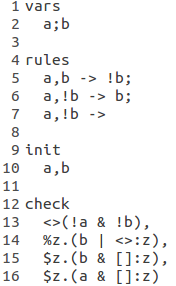
\includegraphics[width=0.33\textwidth]{Figures/modeloMC2-2.png}
  \caption{Ejemplo de descripción MC2 usando azucar sintáctico.}
  \label{fig:MC2-2}
\end{figure}

\begin{figure}[H]
  \centering
  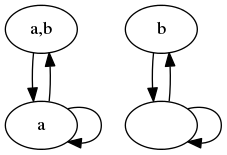
\includegraphics[width=0.4\textwidth]{Figures/kripke5.png}
  \caption{Estructura de Kripke del nuevo modelo.}
  \label{fig:kripke5}
\end{figure}

\begin{figure}[H]
  \centering
  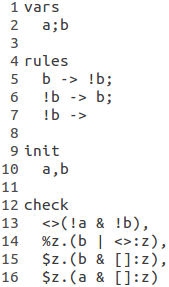
\includegraphics[width=0.33\textwidth]{Figures/modeloMC2-3.png}
  \caption{Ejemplo de descripción MC2 con más de una transición por regla.}
  \label{fig:MC2-3}
\end{figure}

En la sección $check$ se puede ver que hay cuatro propiedades descritas en cálculo-$\mu$, que son las siguientes: $\Diamond (\neg a \land \neg b)$, $\mu z. (b \lor \Diamond z)$, $\nu z. (b \land \Box z)$, y $\nu z. (a \land \Box z)$. Al ejecutar el verificador con la descripción de la figura \ref{fig:MC2-1}, el resultado va a ser el conjunto de propiedades que el modelo haya satisfecho, en este caso $\mu z. (b \lor \Diamond : z)$ y $\nu z. (a \land \Box : z)$, ya que existe un camino en donde $b$ vale en algun momento, y $a$ vale siempre en todo camino. Evidentemente $'\$'$ representa a $\nu$ y $'\%'$ representa a $\nu$. Cabe destacar también que al anteponer $':'$ a una cadena estamos haciendo referencia a una variable y no a una proposición.

\subsection{Semántica formal}

En esta sección vamos a formalizar las nociones descriptas en la sección anterior. Vamos a necesitar usar operaciones de OBDDs, para lo cual tenemos NOT, AND, OR, NULL(True si no hay modelos para este OBDD \cite{Waldmann:6} ), EXISTS, OBDD-TRUE y OBDD-FALSE. La semántica de una descripción MC2 es la siguiente:\\
\\
$[[\ vars\ D\ rules\ C\ init\ E\ check\ P ]]_{m}\ =\ [F\ |\ F \in P\ \land\ NULL\ (NOT\ inst\ E\ ([[F]]_{f}\ [[C]]_{c}\ assoc-init))]$ \\

Es decir, de todas las fórmulas en $P$ solo nos quedamos con aquellas que al instanciarlas con los valores de $init$ siempre da como resultado $True$. La semántica de una declaración está dada por la siguiente función: \\
\\
\begin{align*}
[[p]]_{d}\ &=\ (p,False) \\
[[D0;D1]]_{d}\ &=\ [[D0]]\ ++\ [[D1]] \\
\end{align*}

Una declaración da como resultado un ambiente, es decir, una lista de proposiciones con sus valores asociados ($False$ en principio). A continuación tenemos la función que denota la semántica de los modelos, un modelo es la disyunción de una o más reglas, a su vez, una regla es una disyunción de todas las transiciones que genera, donde una transición es una conjunción de los OBDDs generados por la evaluación de los ambientes del estado corriente y el siguiente (en el siguiente estado todas las proposiciones deben estar primadas).

\begin{align*}
[[C;D]]_{c}\ &=\ [[C]]_{c}\ OR\ [[D]]_{c} \\
[[E0->E1]]_{c}\ &=\ [[E0]]_{e}\ AND\ [[E1]]_{e'} \\
\end{align*}

La evaluación de un ambiente esta dada por las funciones $[[E]]_{e}$ y $[[E]]_{e'}$, donde la única diferencia entre estas funciones es que la segunda prima a las proposiciones. La semántica de un ambiente da como resultado la conjunción de las proposiciones del mismo con paridad acorde a sus valores asociados.

\begin{align*}
[[(p,True)]]_{e}\ &=\ OBDD_{p} \\
[[(p,False)]]_{e}\ &=\ NOT\ OBDD_{p} \\
[[E0++E1]]_{e}\ &=\ [[E0]]_{e}\ AND\ [[E1]]_{e} \\
\end{align*}

\begin{align*}
[[(p,True)]]_{e'}\ &=\ OBDD_{p'} \\
[[(p,False)]]_{e'}\ &=\ NOT\ OBDD_{p'} \\
[[E0++E1]]_{e'}\ &=\ [[E0]]_{e'}\ AND\ [[E1]]_{e'} \\
\end{align*}

Por ultimo, la semántica de las fórmulas, es la vista en el capítulo 3. M es el modelo del sistema (un OBDD). Assoc es una función que asocia cada variable relacional con un OBDD. La operación EXISTS de los OBDD toma un conjunto de variables y las elimina existencialmente de un OBDD.

\begin{align*}
[[p]]_{f}\ M\ assoc\ &=\ OBDD_{p} \\
[[:X]]_{f}\ M\ assoc\ &=\ assoc\ X \\
[[!F]]_{f}\ M\ assoc\ &=\ NOT\ ([[F]]_{f}\ M\ assoc)\\
[[F \& G]]_{f}\ M\ assoc\ &=\ ([[F]]_{f}\ M\ assoc)\ AND\ ([[G]]_{f}\ M\ assoc)\\
[[F | G]]_{f}\ M\ assoc\ &=\ ([[F]]_{f}\ M\ assoc)\ OR\ ([[G]]_{f}\ M\ assoc)\\
[[<>F]]_{f}\ M\ assoc\ &=\ EXISTS\ x'\ :\ M\ AND\ ([[F]]_{f}(x')\ M\ assoc) \\
[[[]F]]_{f}\ M\ assoc\ &=\ [[!<>!F]]_{f}\ M\ assoc \\
[[\%X.F]]_{f}\ M\ assoc\ &=\ FIX\ F\ assoc\ OBDD-FALSE \\
[[\$X.F]]_{f}\ M\ assoc\ &=\ FIX\ F\ assoc\ OBDD-TRUE \\
\end{align*}

\section{Diseño e implementación}

En esta sección vamos a aclarar detalles del diseño y la implementación del verificador de modelos MC2. La herramienta esta implementada en el lenguaje funcional Haskell, y se interpreta con ghc. La misma está compuesta por los módulos $Types$, $Mu$, $MuEval$, $Model$, $ModelEval$, $Main$, y usa dos modulos externos, $OBDD$ \cite{Waldmann:6} (provee la estructura con sus operaciones) y $ParseLib$ \cite{Hutton:10} (tiene utilidades de parsing).

\subsection{Tipos en MC2}

En $MC2$ tenemos proposiciones atómicas ($AP$) representadas por cadenas, cada una tiene asociada un valor lógico ($True$ o $False$), para lo cual existe un tipo $Env$ (ambiente) que consta de una lista de pares de proposiciones atómicas y sus valores lógicos asociados. Un valor de tipo $Env$ representa el estado del sistema en un momento dado. Tambien definimos el tipo $VName$ como sinónimo de cadenas, pero este tipo lo usamos para hacer referencia a variables relacionales. También hemos definido en este modulo el tipo $Assoc$ como una función Assoc: $VName -> OBDD AP$. $OBDD AP$ hace referencia al tipo de OBDDs donde las variables de sus nodos estan representadas con cadenas (AP). Assoc es un tipo que se utiliza en la semántica de las fórmulas de cálculo-$\mu$, este representa una función que toma el nombre de una variable y devuelve el valor asociado (representado por un OBDD).

\subsection{Descripción del modelo en MC2}

Hay dos modulos dedicados a la descripción del modelo. Uno es $Model$, el cuál contiene la definición de la sintaxis de las declaraciones y comandos, y  sus correspondientes $parsers$. El otro módulo es $ModelEval$, este contiene las funciones $ceval$, $deval$ y $eeval$ correspondientes a los evaluadores de comandos, declaraciones y ambientes respectivamente, además de algunas funciones auxiliares. La función $deval$ toma una declaración y un ambiente con proposiciones a inicializar (se usa en la sección $init$ unicamente), y a partir de estos genera el ambiente inicial del sistema. La función $eeval$ transforma un ambiente en una OBDD-conjunción como se vió en la semántica de ambientes.

\subsection{Cálculo-$\mu$ en MC2}

Similarmente tenemos dos modulos dedicados al Cálculo-$\mu$. Uno es $Mu$, el cuál contiene la definición de la sintaxis, y adicionalmente también contiene el $parser$, y un $printer$. El otro módulo es $MuEval$, este contiene la función $check$ que, dada una fórmula, un modelo (OBDD) y la función $Assoc$, evalua la fórmula y devuelve el OBDD correspondiente a su semántica. Al ser funcional la implementación, toda la información necesaria para computar un resultado debe ser pasada como parámetro, por lo que la función $check$ también toma dos parámetros extra, necesarios para reescribir los nombres de las proposiciones atómicas del OBDD por sus respectivas versiones primas (cuando es necesario verificar algo sobre el siguiente estado). Además $MuEval$ contiene algunas funciones auxiliares como $fix$, la cual se utiliza en el cálculo de puntos fijos.

\subsection{Módulo principal}

El módulo $Main$ contiene el $parser$ de descripciones MC2, su evaluador y varias funciones auxiliares para la lectura de archivos.
\chapter{Casos de estudio}

Ya hemos presentado el verificador de modelos MC2 y el lenguaje de descripción asociado al mismo. Es hora de observar algunos ejemplos concretos de uso de esta herramienta, y ese es el propósito de este capítulo final. Veremos como modelar tres clásicos juegos solitarios de lógica y estrategia, y analizaremos hasta que punto es viable describir manualmente el modelo con esta versión básica de MC2.

\section{Cruce del rio}

Existen muchas versiones de este problema, nosotros modelaremos una de las versiones mas conocidas \cite{Hadley:12}. El problema es el siguiente, un granjero va a comprar un zorro, un ganso y una bolsa de frijoles. Mientras vuelve a su casa, se encuentra con que debe cruzar un rio, para lo cuál alquila un bote. El granjero solo puede llevar una de sus compras en el barco. Si se deja al zorro con el ganso, el zorro se lo va a comer, y si se deja al ganso con la bolsa de frijoles, este se va a comer los frijoles. El desafio del granjero es el de llevar todas sus compras intactas al otro lado del rio. El problema consiste entonces en elegir sabiamente que compras trasladar en cada viaje.\\
\\
La descripción MC2 para el modelo de este problema esta en la figura \ref{fig:river}. Para modelarlo declaramos cuatro pares de proposiciones atómicas, uno para cada compra y otro para el barco/granjero, las proposiciones marcadas con $1$ hacen referencia a que estan del lado $origen$ del rio, y las marcadas con $2$ hacen referencia a que estan del lado $destino$ del rio. En cuanto a las reglas, hay dos grupos de reglas a tener en cuenta para describir el comportamiento del sistema, por un lado se describe lo que pasa cuando se dejan juntos objetos incompatibles (por ejemplo, zorro y ganso), por otro lado tenemos las reglas que definen la acción de viajar de un lado del rio al otro (se puede viajar solo o acompañado por un solo objeto). Hay que destacar que, por ejemplo, si $f1$ y $f2$ son falsas significa que los frijoles se han comido, y ninguna regla puede cambiar estos valores. En este caso, en el estado inicial queremos que valga que tanto el granjero/bote como el zorro, el ganso y los frijoles estan del lado $origen$ del rio. Por último, la propiedad que queremos verificar es si existe alguna forma de que, siguiendo las reglas, puedan estar el zorro, el ganso y los frijoles en el lado $destino$ del rio. En la figura \ref{fig:riverobdd} está el OBDD que representa al modelo.

\begin{figure}[H]
  \centering
  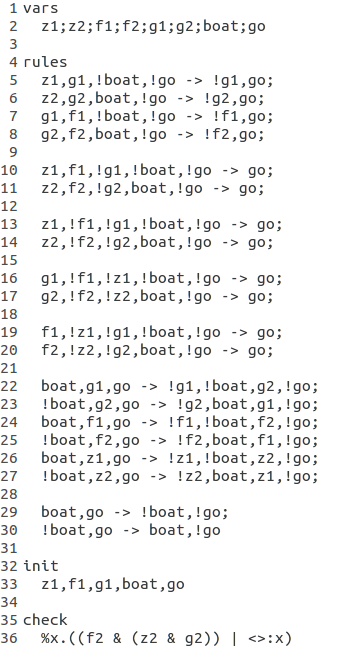
\includegraphics[width=0.6\textwidth]{Figures/rivercross.png}
  \caption{Descripción de modelo del problema del cruce del rio.}
  \label{fig:river}
\end{figure}

\begin{figure}[H]
  \centering
  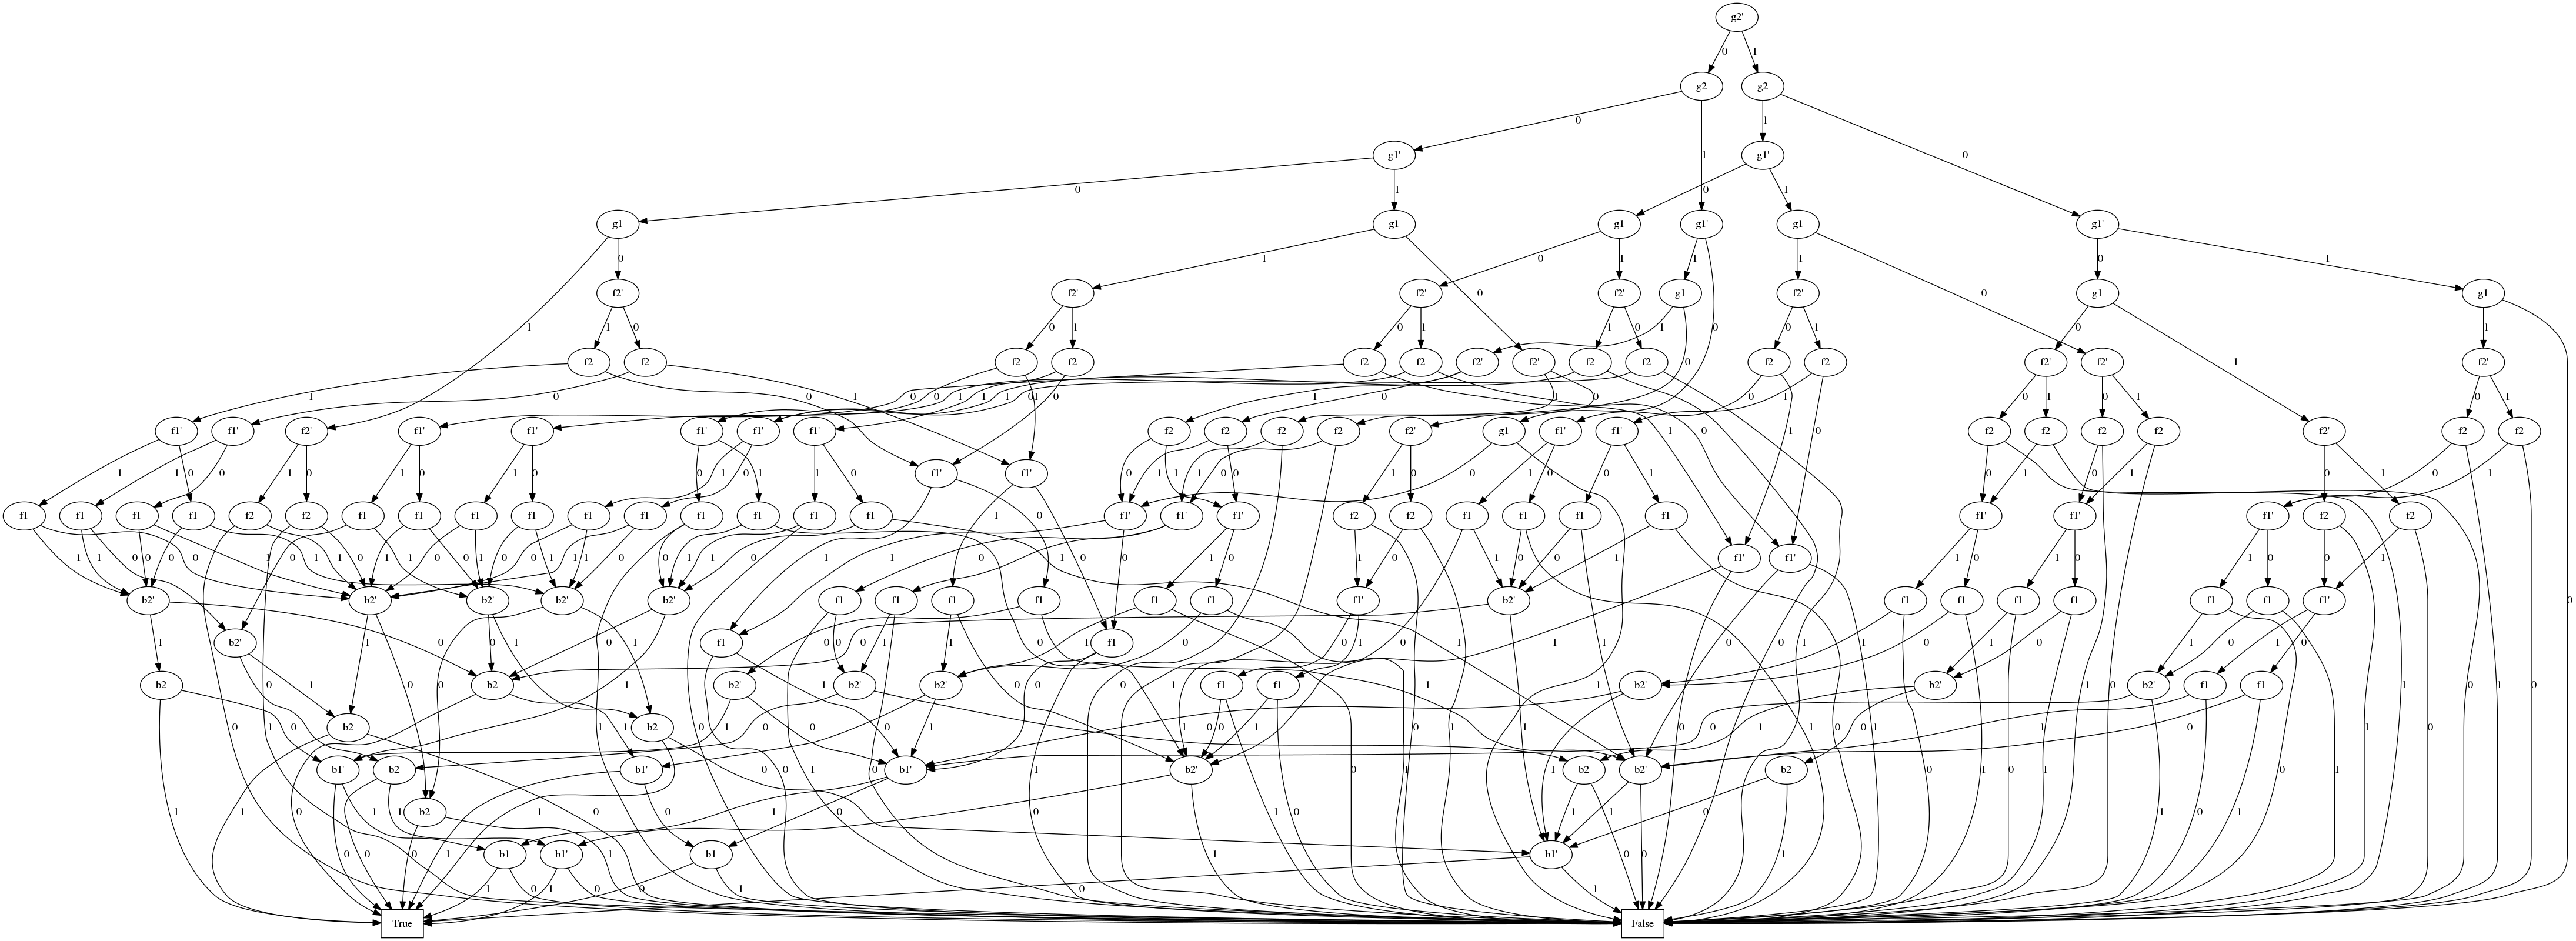
\includegraphics[width=0.9\textwidth]{Figures/riverobdd.png}
  \caption{OBDD para el modelo del cruce del rio.}
  \label{fig:riverobdd}
\end{figure}

\section{1,2,3, Coloca otra vez}

Se parte de una estrella de 5 puntas, ademas de estas, se forman 5 puntos en su interior. Partiendo de uno de los 10 puntos donde no haya una ficha previamente colocada, se cuenta tres posiciones consecutivas sobre una de las aristas que contienen el punto de partida. Tras ello, se coloca una ficha en la tercera posición. En la figura \ref{fig:pentagrama} podemos ver la estrella, hemos nombrado los puntos externos como $o1, ..., o5$ y los internos como $i1, ..., i5$. Por ejemplo partiendo de $o1$ podemos poner una ficha en $i3$ o $i5$. El conteo puede pasar por una posición en la que haya ficha, pero no puede iniciarse en una posición con ficha. El juego estará resuelto cuando se hayan colocado 9 fichas \cite{Juegos:11}. 

\begin{figure}[H]
  \centering
  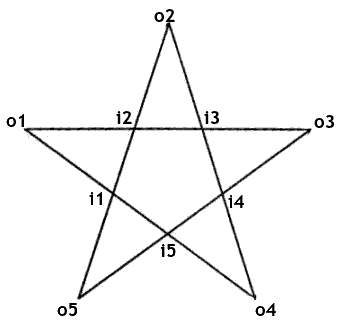
\includegraphics[width=0.5\textwidth]{Figures/pentagram.png}
  \caption{Pentagrama de 1,2,3 Coloca otra vez.}
  \label{fig:pentagrama}
\end{figure}

\noindent En la figura \ref{fig:estrella} se puede ver la descripción MC2 para el modelo de este problema. Para este modelo, declaramos una proposición para cada uno de los diez puntos de la estrella, donde cada proposición es verdadera o falsa dependiendo de si hay o no una ficha en ese punto. Las reglas en este caso representan las jugadas posibles a partir de cada punto. En el estado inicial no hace falta describir nada, ya que inicialmente queremos que no haya ficha en ningun punto de la estrella (todas las proposiciones estan inicializadas en $False$). Por último, la propiedad que queremos verificar es si es posible poner nueve fichas en la estrella, a modo de ejemplo, la formula pide que haya una ficha en todos los puntos excepto $i5$.

\begin{figure}[H]
  \centering
  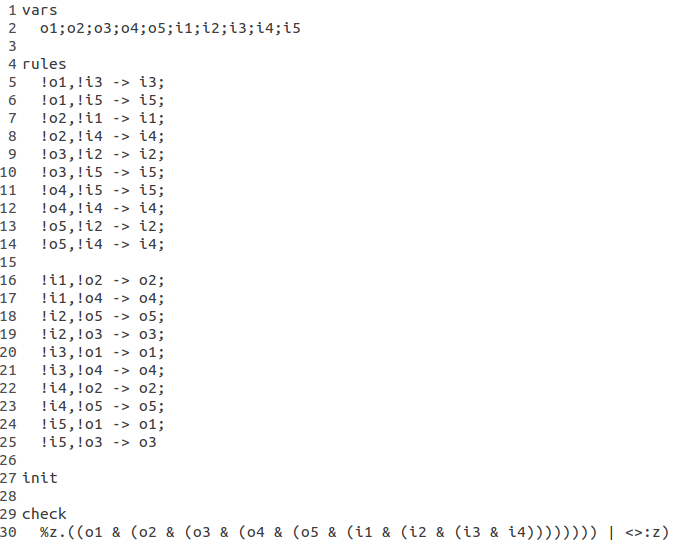
\includegraphics[width=1\textwidth]{Figures/estrella.png}
  \caption{Descripción de modelo del problema de 1,2,3 Coloca otra vez.}
  \label{fig:estrella}
\end{figure}

\section{Ranas saltarinas}

En este juego se tiene una tira de papel dividida en siete casillas \cite{Juegos:11}. La posición inicial es la indicada con tres fichas azules (blancas) y tres rojas (grises) colocadas como en la figura \ref{fig:ranasjuego}. El objetivo del juego consiste en permutar las posiciones de las fichas azules y rojas. Es decir, las azules han de pasar a ocupar las posiciones de las rojas y viceversa. Para ello son válidos los siguientes movimientos:\\
\\
- Una ficha puede moverse a un lugar contiguo, si éste está vacío.\\
\\
- Una ficha junto a otra de distinto color puede saltar por encima de ella si el salto (por encima de una sola ficha) le lleva a una casilla vacía.\\
\\
- Son válidos tanto los movimientos hacia atrás como hacia adelante.\\
\\

\begin{figure}[H]
  \centering
  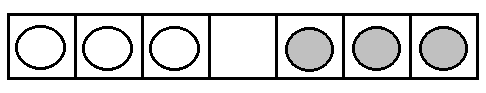
\includegraphics[width=0.8\textwidth]{Figures/ranasjuego.png}
  \caption{Juego de las ranas saltarinas.}
  \label{fig:ranasjuego}
\end{figure}

\noindent La descrición MC2 del modelo para este juego esta en la figura \ref{fig:ranas}. En este caso, tenemos siete proposiciones que representan la ocupación de cada casilla por una ficha roja, y siete más para las fichas azules, es de imaginar que una casilla $i$ esta vacia si $ri$ y $bi$ son falsas, donde $ri$ significa que hay una ficha roja en la casilla $i$, y $bi$ significa que hay una azul en la misma casilla. Las reglas estan divididas en cuatro bloques, dos para cada dirección en la que se puede mover una ficha. Los dos bloques de una dirección representan las primeras dos reglas del juego. Por su puesto, los bloques de la otra dirección son análogos. Como estado inicial tenemos las fichas azules colocadas del lado izquierdo de la tira de casillas, y las rojas del lado derecho, dejando vacia la casilla del medio. Por último, la propiedad que deseamos verificar es si es posible permutar las posiciones de las fichas rojas con las azules y viceversa. 

\begin{figure}[H]
  \centering
  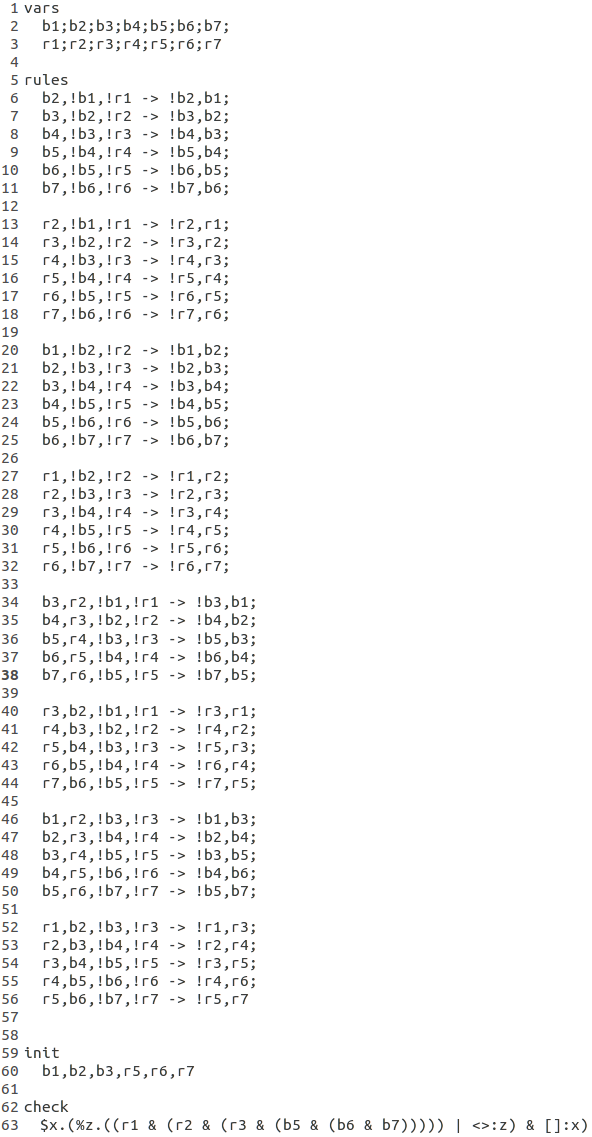
\includegraphics[width=0.5\textwidth]{Figures/ranas.png}
  \caption{Descripción de modelo del problema de las ranas saltarinas.}
  \label{fig:ranas}
\end{figure}

\noindent Nos podemos preguntar como seria la descripción MC2 del modelo si la tira tuviera mas de siete casillas, esta claro que cada vez se vuelve más humanamente inviable a medida que se incrementa el tamaño de casillas. Esto es debido a que la herramienta es de bajo nivel y no cuenta con abstracciones estructurales como los arreglos. Pero es fácil escribir un programa en un lenguaje de alto nivel que genere automáticamente una descripción MC2 para un sistema determinado. En la figura \ref{fig:parser} se puede ver un pseudocódigo para un $parser$ de el problema de las ranas saltarinas para $N$ casillas.

\begin{figure}[H]
  \centering
  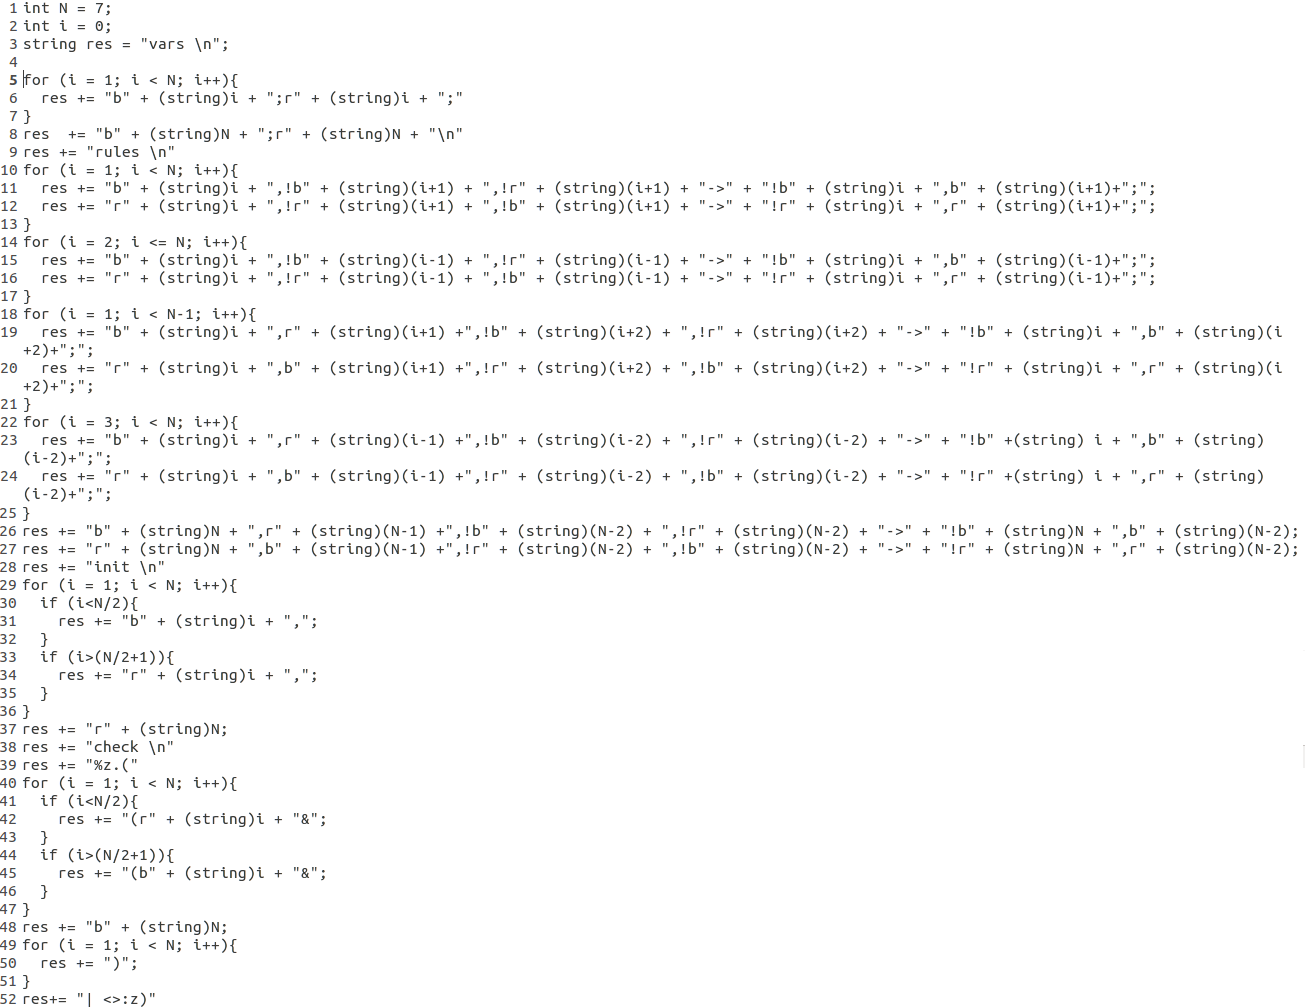
\includegraphics[width=1.1\textwidth]{Figures/parser1.png}
  \caption{Pseudocódigo de $parser$ de alto nivel.}
  \label{fig:parser}
\end{figure}

\chapter*{Conclusión}
\addcontentsline{toc}{chapter}{Conclusión}

Para el desarrollo de esta tesis, se ha investigado sobre la verificación de modelos, sus variantes como la verificación de modelos explicitos y la verificación de modelos simbólicos, para lo cuál tambien fue necesario investigar sobre lógicas temporales para llegar asi a entender el cálculo-$\mu$ y aplicarlo a la práctica.\\
\\
Se logró desarrollar una nueva herramienta de verificación de modelos para cálculo-$\mu$, con un lenguaje de modelado propio basado reglas de construcción de estructuras de kripke, lo que trae algo nuevo a la mesa de verificadores para cálculo-$\mu$ ya existentes como mCRL2 \cite{Groote:14}, TAPAs \cite{Calzolai:15} y CWB \cite{Moller:13}.\\
\\
Como trabajos futuros, se puede considerar la idea de hacer más versatil el lenguaje de modelado, ya sea agregando mas tipos de datos y/o extendiendo las formas de expresar el flujo del sistema que se está modelando.
%% This defines the bibliography file (main.bib) and the bibliography style.
%% If you want to create a bibliography file by hand, change the contents of
%% this file to a `thebibliography' environment.  For more information 
%% see section 4.3 of the LaTeX manual.
\begin{singlespace}
\bibliography{main}
\bibliographystyle{ieeetr}
\end{singlespace}

%\chapter*{Apéndices}
\label{Apendices}
\markboth{Apendices}{} % para que cambie el encabezado, si no, usaría el del último chapter{}
\addcontentsline{toc}{chapter}{Apéndices} % para que se añada en el indice

\appendix
\chapter{Especificación de la Transformación en Query/View/Transformation Relations}
\label{Especificacion de la Transformacion en QVT/Relations QVT}


%\section{Especificación de la Transformación en QVT/ Relations QVT}
%\label{Especificación de la Transformación en QVT/Relations QVT}
Código completo, en QVT Relation, de la transformación de máquinas de estados con elementos opcionales a máquinas de estados concretas.

\begin{verbatim}
-- Inicio de la Transformación 

\end{verbatim}


%Poner el codigo de la transformación por ejemplo

\printindex
\end{document}

